% =====================================================================
% Figure 3 — Spring natural frequency vs. cam harmonics (pgfplots)
% Shows f_{n,out} ≈ 318 Hz and f_{n,in} ≈ 571 Hz against the first
% six cam harmonics (n=1..6) over the engine speed range 0..10 000 rpm.
% Cam runs at half engine speed (4-stroke).
% =====================================================================

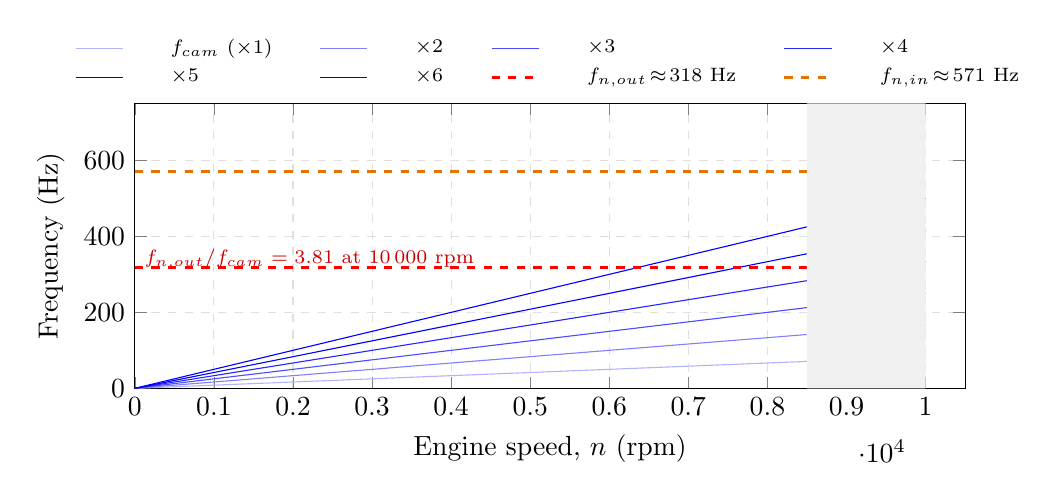
\begin{tikzpicture}
  \begin{axis}[
    width=\linewidth,
    height=5.2cm,
    xlabel={Engine speed, $n$ (rpm)},
    ylabel={Frequency (Hz)},
    xmin=0, xmax=10500,
    ymin=0, ymax=750,
    grid=both,
    grid style={dashed,gray!25},
    legend style={
      at={(0.5,1.02)}, anchor=south,
      legend columns=4,
      font=\scriptsize, draw=none, fill=none,
      column sep=1.5em,
      /tikz/every even column/.append style={column sep=1.5em},
    },
    legend cell align=left,
  ]
  % Cam harmonics: f_h(n) = h * (n_engine / 120). At 10000 rpm: 1*=83.3, 2*=166.7, 3*=250, 4*=333.3, 5*=416.7, 6*=500
  \addplot[domain=0:10000, samples=2, blue!30 ] {x/120};         \addlegendentry{$f_{cam}$ ($\times 1$)}
  \addplot[domain=0:10000, samples=2, blue!50 ] {2*x/120};       \addlegendentry{$\times 2$}
  \addplot[domain=0:10000, samples=2, blue!70 ] {3*x/120};       \addlegendentry{$\times 3$}
  \addplot[domain=0:10000, samples=2, blue!85 ] {4*x/120};       \addlegendentry{$\times 4$}
  \addplot[domain=0:10000, samples=2, blue!95!black] {5*x/120};  \addlegendentry{$\times 5$}
  \addplot[domain=0:10000, samples=2, blue!100!black] {6*x/120}; \addlegendentry{$\times 6$}

  % Spring natural frequencies (constant)
  \addplot[red, dashed, line width=0.9pt, domain=0:10000, samples=2] {318};
  \addlegendentry{$f_{n,out}\!\approx\!318$ Hz}
  \addplot[orange!90!black, dashed, line width=0.9pt, domain=0:10000, samples=2] {571};
  \addlegendentry{$f_{n,in}\!\approx\!571$ Hz}

  % Operating regime shading: 8500-10000 rpm
  \addplot[fill=gray!12, draw=none, forget plot] coordinates {(8500,0) (10000,0) (10000,750) (8500,750)} \closedcycle;

  % 4× rule-of-thumb threshold: 4 * f_cam at engine speed = f_n / 4
  % Annotation
  \node[anchor=west, red!80!black, font=\scriptsize] at (axis cs: 0, 340) {$f_{n,out}/f_{cam}=3.81$ at 10\,000 rpm};

  \end{axis}
\end{tikzpicture}
